\documentclass[12pt,oneside]{uhthesis}
\usepackage{subfigure}
\usepackage[ruled,lined,linesnumbered,titlenumbered,algochapter,spanish,onelanguage]{algorithm2e}
\usepackage{amsmath}
\usepackage{amssymb}
\usepackage{amsbsy}
\usepackage{caption,booktabs}
\captionsetup{ justification = centering }
%\usepackage{mathpazo}
\usepackage{float}
\setlength{\marginparwidth}{2cm}
\usepackage{todonotes}
\usepackage{listings}
\usepackage{xcolor}
\usepackage{multicol}
\usepackage{graphicx}
\floatstyle{plaintop}
\restylefloat{table}
\addbibresource{Bibliography.bib}
% \setlength{\parskip}{\baselineskip}%
\renewcommand{\tablename}{Tabla}
\renewcommand{\listalgorithmcfname}{Índice de Algoritmos}
%\dontprintsemicolon
\SetAlgoNoEnd

\definecolor{codegreen}{rgb}{0,0.6,0}
\definecolor{codegray}{rgb}{0.5,0.5,0.5}
\definecolor{codepurple}{rgb}{0.58,0,0.82}
\definecolor{backcolour}{rgb}{0.95,0.95,0.92}

\lstdefinestyle{mystyle}{
    backgroundcolor=\color{backcolour},   
    commentstyle=\color{codegreen},
    keywordstyle=\color{purple},
    numberstyle=\tiny\color{codegray},
    stringstyle=\color{codepurple},
    basicstyle=\ttfamily\footnotesize,
    breakatwhitespace=false,         
    breaklines=true,                 
    captionpos=b,                    
    keepspaces=true,                 
    numbers=left,                    
    numbersep=5pt,                  
    showspaces=false,                
    showstringspaces=false,
    showtabs=false,                  
    tabsize=4
}

\lstset{style=mystyle}

\title{Meta-Learning para Problemas no Tabulares}
\author{\\\vspace{0.25cm}Roberto García Rodríguez}
\advisor{\\\vspace{0.25cm}Dr. Suilan Estevez Velarde\\\vspace{0.2cm}Lic. Loraine Monteagudo García}
\degree{Licenciado en Ciencia de la Computación}
\faculty{Facultad de Matemática y Computación}
\date{Fecha\\\vspace{0.25cm}\href{https://github.com/Robegr42/thesis}{github.com/Robegr42/thesis}}
\logo{Graphics/uhlogo}
\makenomenclature

\renewcommand{\vec}[1]{\boldsymbol{#1}}
\newcommand{\diff}[1]{\ensuremath{\mathrm{d}#1}}
\newcommand{\me}[1]{\mathrm{e}^{#1}}
\newcommand{\pf}{\mathfrak{p}}
\newcommand{\qf}{\mathfrak{q}}
%\newcommand{\kf}{\mathfrak{k}}
\newcommand{\kt}{\mathtt{k}}
\newcommand{\mf}{\mathfrak{m}}
\newcommand{\hf}{\mathfrak{h}}
\newcommand{\fac}{\mathrm{fac}}
\newcommand{\maxx}[1]{\max\left\{ #1 \right\} }
\newcommand{\minn}[1]{\min\left\{ #1 \right\} }
\newcommand{\lldpcf}{1.25}
\newcommand{\nnorm}[1]{\left\lvert #1 \right\rvert }
\renewcommand{\lstlistingname}{Ejemplo de código}
\renewcommand{\lstlistlistingname}{Ejemplos de código}

\begin{document}

\frontmatter
\maketitle

\begin{dedication}
    A Luis Rodríguez, mi abuelo, a quien debo muchos logros.
\end{dedication}
\begin{acknowledgements}
    A lo largo de este período como estudiante universitario, han sido muchas
    las personas que me han apoyado y ayudado, siendo la base de muchos logros,
    a las cuales quiero dedicar este pequeño espacio, de antemano pido disculpas
    por si se me escapa alguien.
    
    En primer lugar mi familia, el pilar más importante en este trayecto y sin
    la cual nada de esto fuese posible. A mi madre, que siempre me ha apoyado
    mis decisiones; mi abuela, siempre preocupada por mis resultados, algunas
    veces en exceso; a mi hermanita; a mi tío, quién desde la distancia siempre
    estuvo pendiente de mí; a mi padre, quien no pudo estar en estos últimos
    momentos y a Vilmary, quien fue un gran apoyo estos últimos meses, siempre
    haciendo por alegrarme.

    A mis amigos, con los cuales compartí los mejores momentos de esta etapa;
    a mi gran amigo Reinel y a todos los demás que por disímiles situaciones
    no pudieron llegar al final; a Morgado, Manuel y Andrés(el Chino) los
    mejores compañeros de equipo y de fiestas; a Mauro, Jessica, Penelope,
    Adrianna, Lopetegui, Arnel, Darian, Javier Domínguez, David, Henri, Jean
    Pierre y a todos con los que de una forma u otra compartí esta experiencia
    en la universidad.

    También agradecer a mis queridos profesores y alumnos ayudantes, quienes ya
    muchos son profesores también, los cuales, siempre conscientes del esfuerzo
    que exigía la carrera de nosotros, nos alentaban y animaban a no dejar el
    camino; a mis queridos profesores de primer año Celia y Wilfredo, de los
    que tanto disfrute las clases de Álgebra; al profesor Leclerc de quien
    aprendí las nociones básicas de programación; al profesor Somoza, siempre
    con excelentes clases e historias; a la profesora Idania y la ternura con la
    cual enseñaba; a mi querida profesora Alicia con quien tuve el placer de
    compartir un aula dando clases y que tanto me enseñó; a Katrib, Ludwig,
    Naila, Fernando, Alberto, Yudivian, Daniel; en fin, a todos en general.

    Por último y no menos importante, a mis tutores, de los que he sentido un
    gran apoyo y dedicación; a la profesora Suilan y Loraine, por enseñarme
    las maravillas del mundo de la Inteligencia Artificial y al profesor Piad,
    siempre atento y con ganas de enseñar quien además estuvo vinculado a la
    realización de esta tesis.

    Muchas gracias a todos.
\end{acknowledgements}
\begin{opinion}
    En la actualidad el Aprendizaje Automático ha llegado a todas las ramas de
    la industria, ayudando a resolver un gran número de problemas pero creando
    la necesidad de un enorme número de expertos para poder utilizar las
    herramientas adecuadas en cada caso.

    En este escenario el AutoML propone una solución ayudando con la selección
    de forma automática de las mejores soluciones con el problema añadido de
    que incrementa el costo computacional ya que tiene que evaluar muchas
    soluciones para resolver cada problema. Realizando esta tarea cada vez.
    El área de investigación en que incursiona el estudiante propone un enfoque
    para que los sistemas de AutoML puedan aprovechar la información de
    evaluaciones anteriores.

    El  estudiante Roberto García Rodriguez en esta investigación se adentra
    en un tema del estado del arte de gran actualidad y para eso tuvo que
    utilizar conocimientos de varias asignaturas de la carrera y otros que no
    son parte del currículum estándar. Su propuesta implicó estudiar el estado
    del arte de las herramientas de AutoML y su uso en la resolución de
    diferentes tareas. Además implicó conocer una herramienta de AutoML nueva
    e incorporar su estrategia para evaluar y comparar sus resultados en la
    práctica.

    Sus resultados resultan muy prometedores,  permitiendo abrir la puerta a
    resolver problemas de metalearning enl AutoML heterogéneo. Esta mejora es
    considerable para una herramienta del estado del arte, que ya lograba
    resultados comparables a las mejores herramientas de AutoML existentes.
    Más aún, las estrategias desarrolladas en esta investigación han sido
    aplicadas solamente a una parte pequeña del proceso de 
    AutoML pero pueden ser extendidos fácilmente.

    Para poder afrontar el trabajo, el estudiante tuvo que revisar literatura
    científica relacionada con la temática así como soluciones existentes y
    bibliotecas de software que pueden ser apropiadas para su utilización.
    Todo ello con sentido crítico, determinando las mejores aproximaciones y
    también las dificultades que presentan.

    Todo el trabajo fue realizado por el estudiante con una elevada constancia,
    capacidad de trabajo y habilidades, tanto de gestión, como de desarrollo y 
    de investigación.

    Por estas razones recomiendo que le sea otorgado al estudiante Roberto
    García Rodríguez el título de Licenciado en Ciencia de la Computación.

    \begingroup
        \centering
        \wildcard{Dr. Suilan Estevez Velarde}
    \endgroup

\end{opinion}
\begin{resumen}
	Con el desarrollo de la ciencia en el campo de la Inteligencia Artificial,
	la experimentación y el uso de aplicaciones de Aprendizaje de Máquinas
	Automático(AutoML) ha ido en ascenso en los últimos tiempos, llegando a
	campos y ramas de la ciencia tan diversas como la Biología, Neurociencias y
	Medicina, donde han demostrado ser de gran efectividad. A pesar del
	reciente éxito de AutoML, todavía quedan muchos desafíos El uso de
	Meta-learning proporcionará un nuevo camino en la optimización y
	rendimiento de estos programas aprovechando conocimiento ya computado, de
	esta forma se aprende de tareas previamente analizadas, proporcionando una
	idea de solución a futuros	problemas de características semejantes,
	acelerando el proceso de AutoML y obteniendo mejores resultados en el mismo
	período de tiempo. 

	Como sistema de AutoML se escogió AutoGOAL, que destaca por su capacidad de
	generar soluciones eficaces para una amplia gama de dominios, permitiéndole
	resolver una gran cantidad de tareas. La propuesta de meta-learning
	presentada en esta tesis aborda una gran variedad de tareas mediante la
	selección de características capaces de representar el espacio definido por
	ellas.
\end{resumen}

\begin{abstract}
	Resumen en inglés
\end{abstract}
\tableofcontents
\listoffigures
\listoftables
% \listofalgorithms
% \lstlistoflistings

\mainmatter

\chapter*{Introducción}\label{chapter:introduction}
\addcontentsline{toc}{chapter}{Introducción}

En los últimos años se ha hecho creciente el uso, investigación y aplicación
del Aprendizaje de Máquina, en inglés \emph{Machine Learning}~(ML)
~\brackcite{hey2020machinelearning}. Sin embargo, el uso de estás técnicas está
sujeto a conocimiento de mucha teoría matemático-computacional
~\brackcite{dyrmishi2019decision}, lo cual constituye una barrera para nuevos
usuarios~\brackcite{crisan2021fits}. Por ejemplo, para científicos de esta
rama, crear una aplicación de ML está sujeto a la selección de disímiles tipos
de algoritmos~(redes neuronales, modelos bayesianos, algoritmos de
\emph{clustering}, etc) y, a la vez, a ajustar los númerosos hiperparámetros
del algoritmo selecionado. En la mayoría de los casos, a causa del proceso de
prueba y error necesario para encontrar modelos eficientes se invierte una
cantidad enorme de tiempo y recursos en la creación de un modelo que se ajuste
a los requerimientos del problema.

Como consecuencia del costo de empleo de algoritmos y técnicas de ML, surge una
nueva idea para automatizar el proceso de ML, evitando el proceso del costo de
modelación y configuración de los hiperparámetros~\brackcite{thornton2013auto}.
El Aprendizaje de Máquina Automático, en inglés \emph{Automated Machine
Learning}~(AutoML) ha facilitado el proceso de implementación, despliegue,
modelación y desarrollo de algoritmos de ML~\brackcite{paszke2019pytorch}.

El surgimiento de AutoML ha reducido la carga de trabajo de los científicos de
datos y ha permitido una mayor creación de modelos usando algoritmos de ML. De
esta forma se reduce el tiempo de ejecución de procesos, ayudando, además, a no
expertos en el ámbito de la computación. Por lo tanto, AutoML hace accesible
enfoques de aprendizaje automático a los usuarios no expertos que están
interesados en aplicarlos. Con el crecimiento exponencial del poder
computacional y de la cantidad de datos que se generan en la actualidad,
AutoML se ha convertido en un tema de creciente importancia tanto en la
industria como en la academia~\brackcite{he2021automl}.

Aún así existe una carencia en cuanto a reusar conocimiento previamente
generado. Una de las limitaciones presentes en los primeros sistemas de AutoML
es su falta de poder para reusar conocimiento previo para solucionar nuevas
tareas. Para cerrar esta brecha, las herramientas de AutoML comenzaron a
aplicar técnicas de meta-learning, las cuales tienen el objetivo de obtener
modelos para nuevas tareas usando experiencias previas. Meta-learning, o
\emph{aprender a aprender}, es la ciencia de observar sistemáticamente cómo se
desempeñan los diferentes enfoques de aprendizaje automático en una amplia
gama de tareas de aprendizaje, y luego aprender de esta experiencia, o
meta-datos, para aprender nuevas tareas mucho más rápido de lo que sería
posible de otra manera. Esto acelera y mejora drásticamente el diseño
de algoritmos de aprendizaje automático. Además nos permite reemplazar
algoritmos diseñados a mano con enfoques novedosos aprendidos de una manera
basada en datos. Este tipo de estrategias ayudan a disminuir el costo de
aplicar AutoML, al relacionar un nuevo conjunto de datos con los mejores flujos
obtenidos en problemas similares previamente resueltos.\\

\textbf{\Large Problema}\\

A pesar de la creciente cantidad de herramientas de AutoML desarrolladas en los
últimos años, la generación automática de soluciones de ML es
computacionalmente costosa y toma mucho tiempo~\brackcite{crisan2021fits}. Las
razones de estos defectos incluyen un espacio de búsqueda muy grande, tanto
para algoritmos simples de ML como para otras arquitecturas más complejas como
redes neuronales, y que la evaluación de incluso un solo algoritmo en un
conjunto de datos grande puede requerir horas. Esto hace que el proceso de
desarrollo de modelos de ML siga siendo un proceso lento, limitando la
aplicabilidad de AutoML a problemas prácticos en la industria, así como su
potencial para acelerar la investigación científica.\\

\textbf{\Large Motivación}\\

En esta tesis se realiza una propuesta para superar estos obstáculos. El
principal objetivo del enfoque propuesto es asistir a los profesionales de la
industria, a los investigadores en ciencias de datos y de otras ramas de la
ciencia en la selección de modelos incorporando un componente en los
sistemas AutoML, los cuales aumentarán el rendimiento de los mismos, se
acelerarán los procesos de búsqueda proveyendo un conjunto inicial de
algoritmos y las configuraciones de sus hiperparámetros.

Mediante meta-learning, se intenta ganar perspectiva sacada de los meta-datos
de experimentos de aprendizaje automático. Los resultados de cada entrenamiento
son guardados con caracterizaciones del conjunto de datos y sus detalles de
rendimiento, y son usados en las ejecuciones futuras.

Sin embargo, estas herramientas de meta-learning no son suficientemente
flexibles para ser utilizadas en problemas prácticos que requieren la
combinación de algoritmos y tecnologías de diferente naturaleza. Las técnicas
actuales de meta-learning se centran principalmente en un subconjunto
específico de algoritmos, a menudo adaptados a una biblioteca o conjunto de
herramientas.\\

\textbf{\Large Antecedentes}\\

Esta tesis forma parte de las líneas de investigación del grupo de Inteligencia
Artificial de la Facultad de Matemática y Computación de la Universidad de La
Habana. En dicho grupo se ha diseñado el sistema de AutoGOAL, por lo que esta
herramienta es la usada para la incorporación de conocimiento experto mediante
meta-learning. AutoGOAL~\brackcite{autogoal} es un sistema AutoML implementado
como una biblioteca de código abierto en el lenguaje de programación Python.
Utiliza técnicas heterogéneas, que a diferencia de otros sistemas, puede
construir automáticamente flujos de aprendizaje automático que combinen
técnicas y algoritmos de diferentes bibliotecas, incluidos clasificadores
lineales, herramientas de procesamiento de lenguaje natural y redes neuronales.\\

\textbf{\Large Objetivos}\\

El objetivo general de esta tesis es el diseño de una estrategia de
meta-learning para métodos genéricos de AutoML. La estrategia implementada
tendrá el objetivo de acelerar el proceso de búsqueda de AutoML añadiendo
conocimiento previo, de tal manera que se obtengan mejores resultados en el
mismo período de tiempo. Para realizar esto será necesario:

\begin{itemize}
    \item Estudiar diferentes herramientas de meta-learning, así como sistemas
    de Auto-ML presentes en la literatura.
    \item Definir una representación para las soluciones generadas de los
    conjuntos de datos.
    \item Diseñar un algoritmo para recomendar una lista de soluciones para un
    nuevo conjunto de datos basado en estos datos.
    \item Incorporar el conocimiento previo obtenido con meta-learning en
    AutoGOAL para realizar una búsqueda de algoritmos más eficiente.\\
    
\end{itemize}

\textbf{\Large Estructura de la tesis}\\

El resto de la tesis está organizada de la siguiente manera. El Capítulo~
\ref{chapter:state-of-the-art} introduce los problemas de meta-learning y
AutoML y las técnicas que a menudo son aplicadas para tratar con estos
problemas. Esto es seguido por un resumen de los trabajos relacionados con
meta-learning para la selección de algoritmos y de distintas herramientas de
AutoML. Luego, en el Capítulo~\ref{chapter:proposal} se describe la estrategia
de meta-learning propuesta para AutoML, incluyendo un análisis de las
meta-características usadas y las estrategias desarrolladas. En el Capítulo~
\ref{chapter:implementation} se exponen brevemente los aspectos de la
metodología experimental adoptada, se investigan los resultados obtenidos y se
realiza una discusión de los mismos. Posteriormente, se presentan las
conclusiones finales de esta tesis y algunas recomendaciones para estudios
futuros.

\chapter{Estado del Arte}\label{chapter:state-of-the-art}

Este capítulo proporciona una introducción a los campos y los trabajos que
están relacionados con las técnicas utilizadas en esta tesis. Se comienza
introduciendo las ideas básicas de meta-learning
(Sección \ref{section:Metalearning}), definiendo el problema que este campo
resuelve, explicando la estructura de un sistema de meta-learning y varias de
sus aplicaciones. El objetivo fundamental de este trabajo es añadir componentes
de meta-learning a un sistema de Automated Machine Learning (AutoML), así que
este campo es introducido (Sección \ref{section:AutoML}). Se presentan
diferentes formulaciones teóricas del problema de AutoML y se describen los
componentes fundamentales de un proceso de AutoML, así como ejemplos de
sistemas para cada uno de los enfoques existentes. El área de interés de esta
investigación es la aplicación de meta-learning para la selección de modelos,
en concreto, su utilización para añadir conocimiento en sistemas AutoML, por
lo que varias técnicas para la solución de este problema son estudiadas
(Sección \ref{section:MetaAutoML}).

\section{Meta-Learning}\label{section:metalearning}

El término meta-learning ocurrió por primera vez en el área de psicología
educacional. Uno de los investigadores más citados en este campo, John Biggs,
describió meta-learning ``como ser consciente y tomar el control del
conocimiento de uno''~\brackcite{biggs1985role}. Por lo tanto, meta-learning
es visto como un entendimiento y adaptación del aprendizaje en sí en un nivel
más alto que simplemente adquirir conocimiento de una materia. Una persona
consciente y capaz de meta-learning es capaz de evaluar su enfoque de
aprendizaje de acuerdo a los requerimientos de una tarea en específico.

Meta-learning usada en el contexto de aprendizaje automático tiene muchas
similitudes a esta descripción. El conocimiento de una materia se traduce en
\textit{base-learning}, donde la experiencia es acumulada para una tarea en
específico. Meta-learning empieza en un nivel mayor y se encarga de acumular
experiencia sobre varias aplicaciones de un sistema de
aprendizaje~\brackcite{hospedales2021metalearning}.

Debido al creciente poder de computación y gran disponibilidad de conjuntos de
datos en los últimos 20 años, la investigación de aprendizaje automático
enfrentó un creciente número de algoritmos disponibles, incluyendo multitudes
de parametrizaciones, enfoques de pre-procesamiento y pos-procesamiento, así
como una gran variedad de aplicaciones~\brackcite{lemke2013metalearning}.
Promoviendo un mejor entendimiento del aprendizaje automático en sí,
meta-learning puede ser de una ayuda invaluable, evitando procedimientos
extensivos de prueba y error para la selección de algoritmos. Además, puede
permitir entender mejor que hace a un determinado algoritmo desempeñarse bien
en un determinado problema. En esta sección se estudia la definición de
meta-learning, la estructura de un sistema de meta-learning y algunas de sus
aplicaciones.

\subsection{Definición}\label{subsec:meta-definition}

La primera definición de meta-learning en el campo de aprendizaje automático
fue dado por J\"ugen Schmidhuber en 1987, el cual lo considera la interacción
entre agente y el ambiente impulsando la superación personal en el agente.
Meta-learning es mejor entendido comúnmente como ``aprendiendo a aprender'',
lo cual se refiere al proceso de mejorar un algoritmo de aprendizaje a través
de múltiples episodios de aprendizaje. En contraste, el aprendizaje automático
convencional mejora las predicciones del modelo sobre múltiples instancias de
datos. Durante el \textit{base-learning} o aprendizaje base, un algoritmo de
aprendizaje interior (o inferior/base) resuelve una tarea como clasificación
de imágenes, definida por un conjunto de datos y un objetivo. Durante
\emph{meta-learning}, un algoritmo externo (o superior/meta) actualiza el
algoritmo interior de tal manera que el modelo que aprende mejora un objetivo
externo. Los episodios de aprendizaje de la tarea base pueden ser vistos como
una forma de proveer las instancias necesitadas por el algoritmo externo para
aprender el algoritmo de aprendizaje base~\cite{hospedales2021metalearning}.

Meta-learning difiere de \textit{base-learning} en el alcance del nivel de
adaptación. Mientras que el aprendizaje en un nivel base está enfocado en
acumular experiencia en una tarea específica, el aprendizaje en meta-learning
tiene el objetivo de acumular experiencia en el rendimiento de múltiples
aplicaciones de un sistema de aprendizaje. De esta forma, muchos algoritmos
convencionales tales como la búsqueda aleatoria de hiperparámetros mediante
validación cruzada podrían caer en la definición de meta-learning. La
característica destacada del \emph{meta-learning} contemporáneo es un
meta-objetivo explícitamente definido, y una optimización de extremo a extremo
del algoritmo interior con respecto a este objetivo.

\subsection{Campos relacionados}\label{subsec:meta-related-fields}

Aquí se posiciona meta-learning contra áreas relacionadas cuya relación con
meta-learning es a menudo una fuente de confusión
\brackcite{hospedales2021metalearning}:

\begin{description}
	\item[Transfer Learning (TL):] TL usa experiencia pasada de una tarea
    fuente para mejorar el aprendizaje (la velocidad, la eficiencia de los
    datos, la precisión) de una tarea destino. TL se refiere a esta área de
    problemas como familia de soluciones, y para su solución hace uso de la
    transferencia de parámetros, más el ajuste opcional de los mismos. En
    contraste, meta-learning se refiere al paradigma que puede ser utilizado
    para mejorar TL, así como otros problemas. En TL el modelo final es
    extraído por aprendizaje simple en la tarea fuente sin el uso de un
    meta-objetivo. En meta-learning, el modelo final estaría definido por la
    optimización externa que evalúa el beneficio del modelo cuando aprende una
    nueva tarea.
	
	\item[Aprendizaje multi-tarea (MTL):] intenta aprender en conjunto algunas
    tareas relacionadas para beneficiarse de la regularización debido al
    intercambio de parámetros y la diversidad de la representación compartida
    resultante. Como TL, MTL convencional es una optimización de un solo nivel
    sin un meta-objetivo. Además, el propósito de MTL es el de aprender de una
    cantidad fija de tareas conocidas, mientras que el objetivo de
    meta-learning es a menudo aprender de tareas futuras no vistas.
	 
	\item[Optimización de Hiperparámetros (HPO):] está dentro de las
    consideraciones de meta-learning, en el sentido de que hiperparámetros como
    la tasa de aprendizaje o la fuerza de regularización describen
    ``cómo aprender''. Aquí se suelen incluir tareas de HPO que definen un
    meta-objetivo que es entrenado de extremo a extremo con redes neuronales,
    tales como el aprendizaje de hiperparámetros basados en gradientes y la
    búsqueda de arquitectura neuronal. Pero excluyen otros enfoques como
    búsqueda aleatoria y optimización bayesiana, las cuales raramente están
    consideradas como meta-learning~\brackcite{hospedales2021metalearning}.
	
	\item[AutoML:] AutoML es más bien un espectro amplio de enfoques con el
    objetivo de automatizar partes del proceso de aprendizaje automático que
    son típicamente manuales, tales como la preparación de los datos, la
    selección de algoritmos, ajuste de hiperparámetros, y búsqueda de
    arquitecturas. AutoML a menudo utiliza numerosas heurísticas afuera del
    alcance de meta-learning, y se usa en tareas como limpieza de datos, que
    son menos importantes en meta-learning. Sin embargo, AutoML a veces
    utiliza optimizaciones de extremo a extremo de un meta-objetivo, así que
    meta-learning puede ser visto como una especialización de AutoML. AutoML
    a menudo usa técnicas de meta-learning para inicializar su proceso de
    optimización y ganar experiencia de experimentaciones pasadas.
\end{description}

\subsection{Estructura de un Sistema de Meta-Learning}

Un sistema de meta-learning está compuesto esencialmente por dos partes. Una
parte tiene la tarea de adquirir meta-conocimiento de sistemas de aprendizaje
automático. La otra parte tiene el objetivo de aplicar este meta-conocimiento
a nuevos problemas con el objetivo de identificar un algoritmo o técnica de
aprendizaje óptimo.

\subsubsection{Adquisición de Meta-Conocimiento} 

Hay dos modos naturales en los cuales el meta-conocimiento puede ser adquirido.
Una posibilidad es depender de conocimiento experto y otra posibilidad es usar
un procedimiento automático. 

La obtención de meta-conocimiento a través del conocimiento experto se realiza
en la forma de reglas que coinciden con las características de dominio
(conjunto de datos) y con algoritmos de aprendizaje automático. Estas reglas
pueden ser hechas a mano, teniendo en cuenta resultados teóricos, el
conocimiento humano y evidencia empírica. Sin embargo, este método tiene serias
desventajas: el conjunto de reglas resultantes probablemente esté incompleto y
el mantenimiento del conjunto de reglas a medida que nuevos algoritmos se
vuelven disponibles es problemático. Como resultado, la mayoría de la
investigación se ha enfocado en métodos automáticos
~\cite{bradzil2017metalearning}.
	
Para la automatización de la adquisición de conocimiento es necesario un
conjunto de problemas y un conjunto de algoritmos de aprendizaje automático
que queremos considerar. Entonces se necesita definir un método experimental
que determine con cuáles alternativas deberíamos experimentar y en qué orden.
Por ejemplo, dado un conjunto de datos (con ciertas características) y
ciertos algoritmos de aprendizaje automático, se producen resultados de
rendimiento para cada uno de estos algoritmos a través de un método de
evaluación (como validación cruzada). Los resultados y la estructura de los
algoritmos aplicados, junto con la caracterización de los conjuntos de datos,
representan un pedazo de información que es guardado en una base de
meta-conocimiento. El proceso es entonces repetido para otras combinaciones de
conjuntos de datos y algoritmos. 
En la Figura~\ref{fig:adquisition} se muestra cómo se realiza el proceso de
adquisición del meta-conocimiento.

\begin{figure}[H]
    \centering
    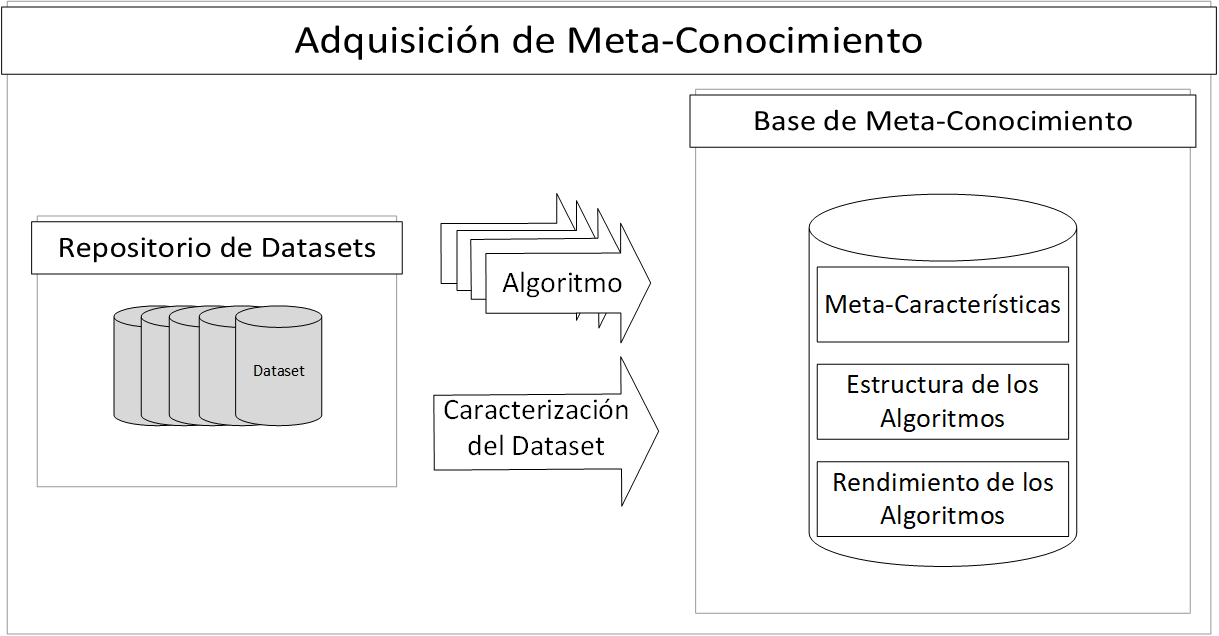
\includegraphics[scale=.5]{Figures/adquisition.png}
    \caption{Proceso de adquisición de meta-conocimiento. }
    \label{fig:adquisition}
\end{figure}

\subsubsection{Aplicación de Meta-Conocimiento}

En un sistema de meta-learning la aplicación de meta-conocimiento puede ser
usada para ayudar a seleccionar o adaptar algoritmos de aprendizaje automático.
Por ejemplo, se puede considerar nuestro problema de la selección de algoritmos
de aprendizaje automático dado un determinado conjunto de algoritmos. Este
puede ser visto como un problema de búsqueda, donde el espacio de búsqueda
incluye los algoritmos de aprendizaje automático individuales y el objetivo es
identificar el mejor algoritmo. Este proceso puede ser dividido en dos fases
separadas. La Figura~\ref{fig:application} muestra un diagrama de como ocurre
este proceso.

En la primera fase (Figura~\ref{fig:application} a) el objetivo es identificar
un subconjunto adecuado de algoritmos de aprendizaje automático basados en un
conjunto de datos de entrada. El método de selección empleado en ese proceso se basa en
el meta-conocimiento. Dado un nuevo conjunto de datos sus meta-características son
extraídas y estas son analizadas para extraer de la base de meta-conocimiento
los conjunto de datoss similares. Por lo general, el resultado de esta fase es
representado en la forma de un subconjunto rankeado de algoritmos de
aprendizaje automático.

La segunda fase (Figura~\ref{fig:application} b) tiene el objetivo de buscar a
través del espacio reducido. Cada opción es evaluada empleando una métrica de
rendimiento determinado (por ejemplo, \textit{accuracy}). Usualmente, la
validación cruzada es usada para identificar el mejor algoritmo de aprendizaje.
Es necesario notar que el meta-conocimiento no elimina completamente la
necesidad del proceso de búsqueda, sino que proporciona una búsqueda más
efectiva. La efectividad de la búsqueda depende de la calidad del
meta-conocimiento~\brackcite{bradzil2017metalearning}.


\begin{figure}[H]
	\centering
	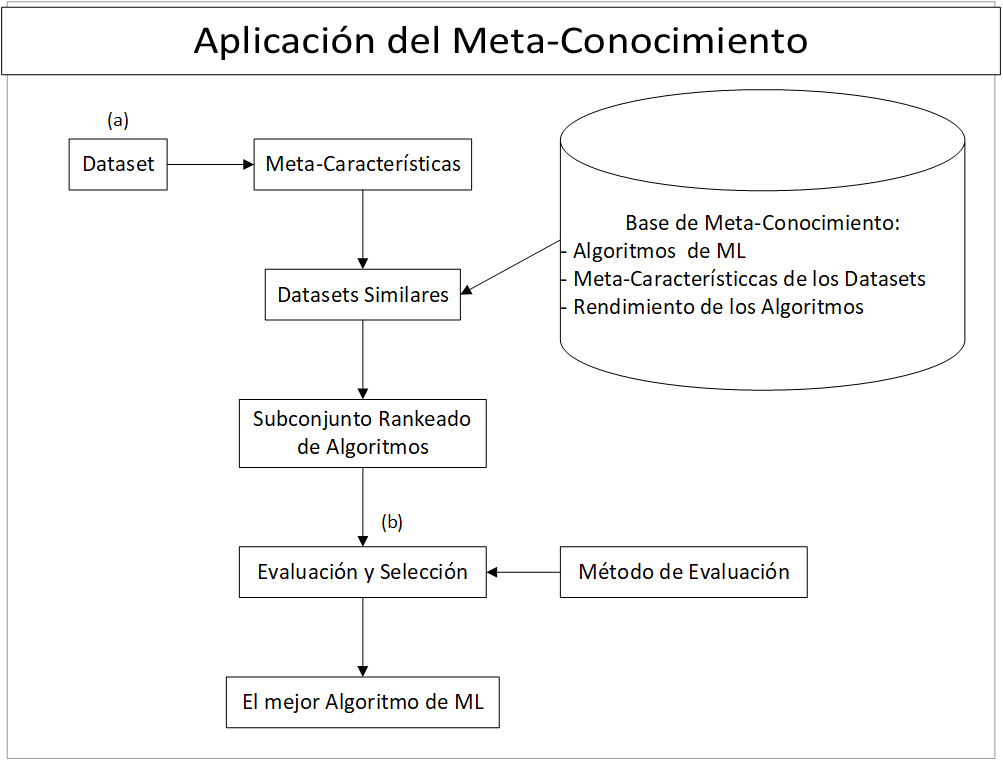
\includegraphics[scale=.5]{Figures/application.png}
	\caption{Proceso de aplicación de meta-conocimiento.}
	\label{fig:application}
\end{figure}

\subsection{Aplicaciones de Meta-Learning}\label{subsec:mtl_aplications}

Meta-learning puede ser empleada en una variedad de configuraciones, con cierto
desacuerdo en la literatura sobre lo que constituye exactamente un problema de
meta-learning. Meta-learning es extremadamente útil en los casos donde es
requerido un modelo de aprendizaje automático y hay poca cantidad de datos,
ya que el modelo contiene muchos parámetros que no pueden ser estimados
precisamente con pocos datos. Algunas de las aplicaciones comunes son en la
investigación robótica, donde se espera que los robots tengan un mayor nivel
de autonomía en IA, en el descubrimiento de drogas para manejar los datos de 
altas dimensiones con un tamaño de muestra pequeño y en la traducción de
lenguajes raramente usados~\brackcite{peng2020comprehensive}.

Meta-learning constituye una solución factible para los problemas donde una
definición específica de ``tarea'' y ``etiqueta'' puede ser claramente
distinguida. Un sistema de meta-learning es flexible y puede ser
integrado convenientemente con la mayoría de los algoritmos de aprendizaje
automático para proporcionar soluciones factibles~\brackcite{peng2020comprehensive}.
Para las tareas que son computacionalmente costosas, meta-learning presenta la
opción de agregación o adaptación de los resultados anteriores para salvar
recursos computacionales.

\section{AutoML}\label{section:AutoML}

\textit{Automated Machine Learning} (AutoML) o Aprendizaje de Máquinas
Automático es el campo que se enfoca en los métodos que tienen el objetivo de
automatizar diferentes etapas del proceso de aprendizaje automático. Como su
nombre indica, AutoML es la intersección de dos campos: automatización y ML.
Las soluciones de AutoML están recibiendo incrementalmente más atención tanto
por la comunidad de ML como por los usuarios por las grandes cantidades de
datos disponibles en todas partes y la falta de expertos de aprendizaje
automático que puedan supervisar/asesorar el desarrollo de sistemas basados en
ML~\brackcite{hutter2019autmlbook}.

La diferencia entre el aprendizaje automático clásico y AutoML es que en el
primero, los humanos están grandemente involucrados en la configuración de las
herramientas de aprendizaje realizando ingeniería de características, selección
y evaluación de modelos. Como resultado, los humanos realizan la mayor parte
del trabajo en las prácticas del aprendizaje automático. Sin embargo, en
AutoML, todo esto puede ser hecho con programas de forma automática.

La comunidad de AutoML se ha centrado en resolver varias partes de un flujo de
trabajo de aprendizaje automático estándar. Algunos ejemplos de estas partes o
subtareas que son aplicadas en AutoML son:

\begin{description}
	\item[\textit{Automated Data Preparation} o Preparación Automática de
    Datos:] el flujo de trabajo de la preparación de datos está compuesto por 
    3 componentes: colección de datos, limpieza de datos e incremento de datos.
    La colección de datos es un paso necesario para construir un nuevo conjunto
    de datos o extender el conjunto de datos existente. El proceso de limpieza
    de datos es usado para filtrar los datos con ruido para que el
    entrenamiento del modelo no sea comprometido. El incremento de datos tiene
    un rol importante en mejorar la robustez del modelo y mejorar su
    rendimiento. Este paso es uno de los que más difícilmente son
    automatizados~\brackcite{he2021automl}.
	
	\item[\textit{Automated Feature Engineering} o Ingeniería Automática de
    Características:] el objetivo de ingeniería de características es construir
    más características para mejorar el rendimiento de aprendizaje cuando las
    características no son lo suficientemente informativas. Para esto se diseña
    un modelo que aprende de las características de entrada para construir
    nuevas características, con las cuales el algoritmo de aprendizaje
    automático obtiene un mejor rendimiento. Con la automatización de esta
    tarea se elimina parte de la asistencia humana para construir
    automáticamente nuevas características~\brackcite{he2021automl}.
	
	\item [\textit{Neural Architecture Search} (NAS) o Búsqueda de
    Arquitecturas Neuronales:] el objetivo de NAS es encontrar una arquitectura
    de redes neuronales profundas con buen rendimiento en un conjunto de datos
    determinado. NAS ha sido usado para diseñar redes que están a la par o
    tienen mejores resultados que arquitecturas diseñados a man
    ~\brackcite{zoph2017learning, witsuba2019nas}. Aunque es una práctica común
    optimizar la arquitectura y las configuraciones de los hiperparámetros en
    secuencia, existe evidencia reciente de que deberían ser optimizadas en
    conjunto \brackcite{bischl2021hyperparameter}.
\end{description}

Sin embargo, los estudios recientes de AutoML buscan automatizar el flujo de
algoritmos de aprendizaje automático entero~\brackcite{fuerer2015efficient,
paszke2019pytorch}. Un flujo de algoritmos es una forma de codificar y
automatizar el flujo de trabajo necesario para producir un modelo de
aprendizaje automático. Los flujos de algoritmos de aprendizaje automático
constan de varios pasos secuenciales que realizan desde la extracción de datos
y el preprocesamiento hasta el entrenamiento y la implementación del modelo
~\cite{web-mlpipe}.

\subsection{Definición del problema}\label{subsec:automl_problem_definition}

Dos problemas importantes en AutoML son que ningún algoritmo de ML obtiene los
mejores resultados en todos los conjunto de datoss, también conocido como
\textit{No Free Lunch Problem} \cite{wolpert1995no}, y que algunos métodos de
aprendizaje automático dependen crucialmente de la optimización de
hiperparámetros. Para la resolución de estos problemas AutoML se apoya de dos
áreas o subtareas que constituyen su base: la selección de modelos
(\textit{Model Selection}, MS)~\cite{thornton2013auto} y la optimización de
hiperparámetros (\textit{Hyperparameter Optimization}, HPO)
~\cite{fuerer2019hyperparameter}. La combinación de estas áreas se refiere al
problema de AutoML como un problema de selección combinada de modelos y
optimización de hiperparámetros (\textit{Combined Algorithm Selection and
Hyperparameter Optimization}, CASH)~\cite{thornton2013auto}.

\subsubsection{Selección de Modelos}

El objetivo de la selección de modelos es encontrar un algoritmo de aprendizaje
automático adecuado para un conjunto de datos determinado. Hay muchos aspectos de los
cuales un científico de datos se preocupa en la selección de algoritmos, tales
como la complejidad computacional, diferencias en el tiempo de entrenamiento y
si el algoritmo permite una entrada no lineal, y es útil considerar estos
aspectos en la automatización. Para realizar esta tarea un sistema AutoML
realiza una búsqueda sobre un conjunto de algoritmos disponibles, con el
objetivo de determinar cuáles de ellos pertenecen al flujo óptimo de un
problema determinado~\cite{li2021automl}.

\subsubsection{Optimización de Hiperparámetros}

Los algoritmos de aprendizaje automático son altamente configurables por sus
hiperparámetros (HP). Estos últimos a menudo influencian substancialmente el
comportamiento y la velocidad del algoritmo y tienen que ser seleccionados con
cuidado con el objetivo de alcanzar un rendimiento óptimo. Tanto para expertos
como para no expertos, ajustar los hiperparámetros para optimizar el
rendimiento del modelo puede ser una tarea difícil y tediosa, a menudo es
bastante costosa y propensa a errores, especialmente cuando son seleccionados
en un proceso de prueba y error. Los algoritmos de optimización de
hiperparámetros (HPO) identifican automáticamente una configuración de
hiperparámetros (HPC) buena para un algoritmo de ML, reduciendo así el esfuerzo
humano. Por lo tanto, una de las tareas fundamentales de AutoML es ajustarlos
para optimizar el rendimiento de los algoritmos de ML~\cite{li2021automl}.

\section{Meta-Learning en AutoML}\label{section:meta-with-AutoML}

La principal área de investigación de meta-learning estudiada en este trabajo
es la selección de algoritmos, la cual ha recibido una considerable cantidad
de investigación. En el caso especial de meta-learning, el aspecto de interés
es la relación entre las características de los datos y el rendimiento del
algoritmo, con el objetivo final de predecir un algoritmo o un conjunto de
algoritmos adecuado para un problema específico. Como motivación está el hecho
de que es inviable examinar todas las posibles alternativas de algoritmos en un
procedimiento de prueba y error. La aplicación de meta-learning en este campo
puede, por lo tanto, ser útil tanto para proveer una recomendación para un
usuario final como de paso preliminar para recomendar algoritmos a soluciones
más costosas computacionalmente, como los algoritmos de optimización usados en
herramientas de AutoML. 

El desafío en meta-learning para la selección de modelos es aprender de
experiencias pasadas de una forma sistemática e impulsada por los datos.
Primero, es necesario extraer los meta-datos que describen las tareas de
aprendizaje anteriores y los modelos previamente aprendidos. Estos meta-datos
comprenden las configuraciones exactas de los algoritmos empleados para
entrenar los modelos, incluyendo:

\begin{itemize}
	\item Las configuraciones de los hiperparámetros, composiciones de los
    flujos de algoritmos y/o arquitecturas de redes neuronales.
	\item Las evaluaciones del modelo resultante, tales como la precisión y el
    tiempo de entrenamiento.
	\item Propiedades medibles de la tarea en sí, que son extraídas de los
    conjuntos de datos, también conocidas como meta-características.
\end{itemize}

Luego es necesario aprender de estos meta-datos previos, para extraer y
transferir conocimiento de la búsqueda de los modelos óptimos para nuevas
tareas. El resto de esta sección presenta una visión general de diferentes
enfoques de meta-learning para hacer esto efectivamente. Además, se muestran
ejemplos de cómo estos enfoques han sido utilizados como paso preliminar en
varias herramientas de AutoML.

\subsection{Meta-Características}

Cómo extraer información adecuada para caracterizar tareas específicas es una
de las preguntas fundamentales en meta-learning. Investigadores han intentado
contestar esta pregunta observando las características de los conjuntos de datos
que afectan el rendimiento de los algoritmos~\cite{Rivolli2018TowardsRE}. Estas
caracterizaciones son denominadas meta-características y usualmente se
encuentran divididos en cinco grupos. Estos grupos son subconjuntos de medidas
de caracterización \cite{bradzil2009metalearning} que comparten similitudes
entre ellas:

\begin{description}
	\item[Simple:] son características que son fácilmente extraídas de los
    datos, son conocidas comúnmente y no requieren recursos computacionales
    significativos. Representan información básica sobre el conjunto de datos.
    Hasta un determinado punto son concebidas para medir la complejidad del
    problema subyacente. Algunas de las caracterizaciones incluidas en este
    grupo son: el número de instancias, el número de atributos, la
    dimensionalidad del conjunto de datos, la proporción de valores faltantes,
    etc. También son llamadas medidas \textit{generales}.
	
	\item[Estadísticas:] son características que capturan las propiedades
    estadísticas de los datos. Estas métricas capturan los indicadores de
    distribución de datos, tales como la media, la desviación estándar,
    la correlación y curtosis. Solo caracterizan los atributos numéricos. Las
    caracterizaciones estadísticas son deterministas y algunas de ellas
    requieren la definición de valores de hiperparámetros.
	
	\item[Teóricas de la información:] son características del campo de teoría
    de la información. Estas medidas están basadas en la entropía, la cual
    captura la cantidad de información en los datos y su complejidad. Ellas
    pueden ser usados para caracterizar los atributos discretos. Además, son
    computadas directamente, libres de hiperparámetros, deterministas y
    robustas. Semánticamente, describen la variedad y la redundancia de los
    atributos utilizados para representar las clases.
	
	\item[Basados en modelos:] son características extraídas de un modelo
    inducido de los datos de entrenamiento. Las características en este grupo
    están caracterizadas por la extracción de información de un modelo de
    aprendizaje de predicción, generalmente, un árbol de decisión. Las medidas
    caracterizan la complejidad de los problemas basados en las hojas, los
    nodos y la forma del árbol. Están diseñadas para caracterizar problemas
    supervisados, todas las medidas son deterministas, robustas y requieren la
    definición de los hiperparámetros que hay en el algoritmo de árboles de
    decisión para inducir el modelo.
	
	\item[\textit{Landmarking}:] son características que usan el rendimiento de
    algoritmos de aprendizaje simples y rápidos para caracterizar los conjunto
    de datoss. Los algoritmos deben tener diferentes sesgos y capturar
    información importante con un costo computacional bajo. Las medidas
    caracterizan problemas supervisados y son indirectamente extraídas.
    Requieren la definición de hiperparámetros: el algoritmo de aprendizaje,
    la medida de evaluación usada para comprobar el rendimiento del modelo y
    el procedimiento empleado para calcularla (por ejemplo, validación cruzada).
\end{description}

Los primeros tres grupos representan los enfoques más comunes y tradicionales
de las caracterizaciones de los datos. Los últimos dos requieren el uso de
algoritmos de aprendizaje automático, porque extraen la complejidad del modelo
o medidas de rendimiento del mismo, haciéndolos además más complejos.

\section{Conclusión}\label{sec:conclusion}

La democratización de la Inteligencia Artificial es una de las preocupaciones
fundamentales, tanto de la comunidad científica como de los expertos de la
industria. El campo del AutoML se presenta como una alternativa prometedora
para disminuir substancialmente el esfuerzo que conlleva la aplicación de
técnicas de inteligencia artificial, y específicamente de aprendizaje
automático, a problemas concretos. Por otro lado, el campo de meta-learning
aplicado a AutoML permite reusar conocimiento previo para solucionar nuevas
tareas. Este tipo de estrategias ayuda a disminuir el costo de aplicar AutoML,
al relacionar un nuevo conjunto de datos con los mejores flujos obtenidos en
problemas similares previamente resueltos. La habilidad de los sistemas de
computación de guardar virtualmente grandes cantidades de experiencias pasadas
de aprendizaje (en forma de meta-datos) abre una gran cantidad de oportunidades
de usar esa experiencia en maneras completamente diferentes
~\cite{vanschoren2018metalearning}.

Aunque existen varias herramientas de meta-learning que han sido exitosas al
aplicarse a AutoML resolviendo problemas específicos de inteligencia
artificial, estas herramientas son aún demasiado rígidas para ser utilizadas
en problemas prácticos que requieren la combinación de algoritmos y tecnologías
de diferente naturaleza. Por lo tanto, la herramienta de meta-learning creada
tiene el objetivo de abordar una gran variedad de problemas mediante la
selección de meta-características capaces de representarlas. Además, es
necesario el uso de un sistema complementario de AutoML capaz de generar
soluciones eficaces para una amplia gama de tareas y dominios. Por esta razón,
se utiliza de AutoGOAL\brackcite{estevanellhacia}, que destaca por su
capacidad de abordar diferentes dominios combinando de forma transparente
técnicas y herramientas dispares. AutoGOAL usa como método de optimización
\textit{Probabilistic Grammatical Evolution}~\cite{estevez2021general} (PGE),
que no había sido usado anteriormente junto con meta-learning, lo que añade
complejidad a la propuesta. El uso de esta estrategia de meta-learning
permitirá disminuir el costo de aplicar AutoML y generalizar AutoML a dominios
novedosos.

\chapter{Propuesta}\label{chapter:proposal}

%La propuesta se centra en una propuesta de metalearning sobre el espacio de busqueda y utilizar el conocimiento generado por otros usuarios

La propuesta de meta-learning implementada se centra en un análisis sobre
una descripción de problemas, definiendo como espacio de búsqueda los elementos
característicos de los mismos. Dicho análisis se realiza sobre conocimiento
previo, generado por los usuarios, el cual, en los sistemas clásicos de AutoML
es desechado, causando la pérdida de los mismos y la necesidad de un
reentrenamiento de los modelos en futuros análisis.

Por lo tanto, la propuesta hecha surge de la necesidad del reaprovechamiento
del conocimiento generado en un momento dado, el cual servirá para
procesamientos de problemas venideros, obteniendo una mejora en cuanto a costo
temopral de los procesamientos sin la necesidad de recomputar soluciones
enteras desde un principio.

%COncretar el enfoque de la propuesta, que aprovecho de los usuarios anteriores.
%Importa el problema e importa los pipeline evaluados

Dicha propuesta se basa entonces en guardar características que describan los
conjuntos de datos, igualmente se salvan las soluciones más prometedoras, las
cuales se obtuvieron de análisis previos de dichos conjuntos de datos. Estas
características servirán para representar similitud entre problemas y
relacionar las soluciones con mayor posibilidad de encajar en los mismos, de
esta forma se gana en tiempo de ejecución de una solución y se evita la
exploración de soluciones no factibles.

%Diagrama de la propuesta 

\section{Diagrama de la Propuesta}

%Explicar el diagrama, explicar el flujo

El flujo de ejecución de la propuesta consta de varios pasos, como se muestra
en la Figura \ref{fig:prop-flow}.

\begin{figure}[H]
    \centering
    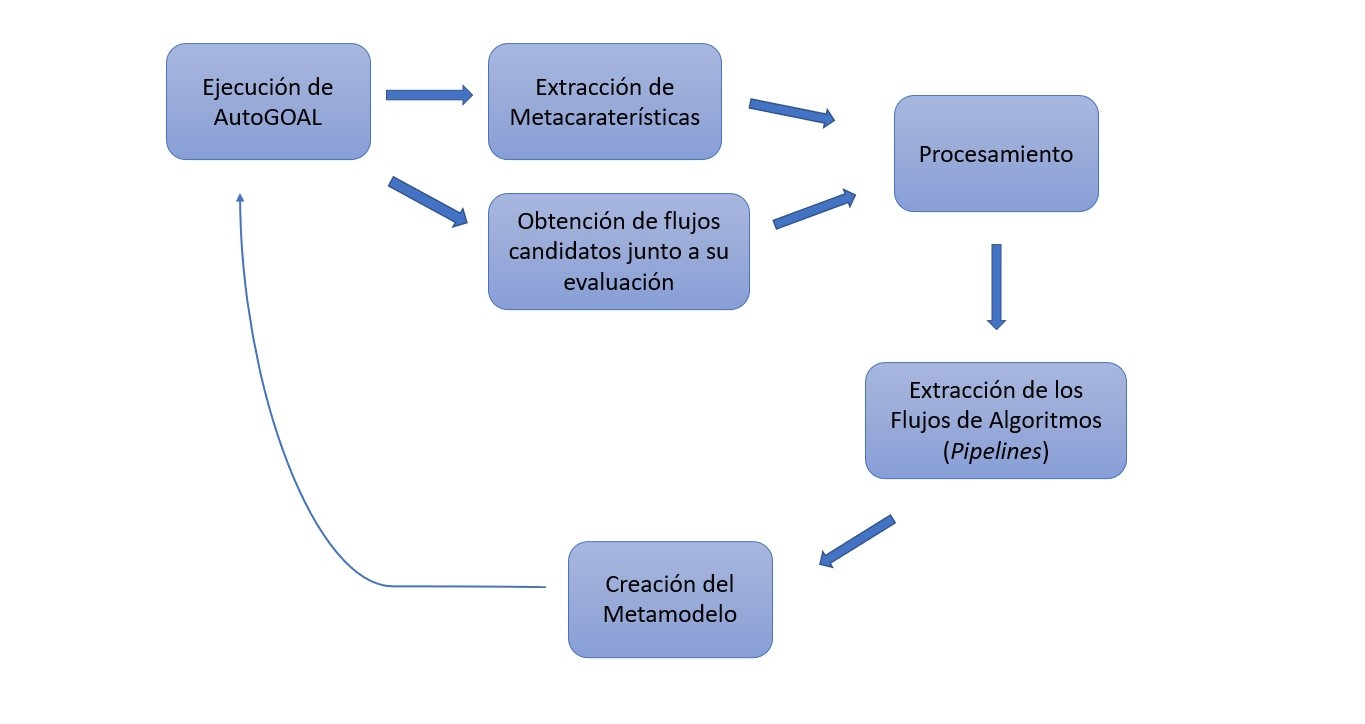
\includegraphics[scale=.5]{Figures/proposal-flow.jpg}
    \caption{Esquema del flujo la propuesta}
    \label{fig:prop-flow}
\end{figure}

Primeramente se realiza una ejecución de AutoGOAL(sistema de AutoML usado en el
trabajo), con lo cual el sistema va a entrenarse en varios conjuntos de datos.
Luego se extraen características distintivas de estos problemas y se
seleccionan los flujos de algoritmos mejor ajustados al problema, medidos por
el resultado de efectividad que ofrecen. Posteriormente se procesan todos estos
datos los cuales servirán para un metamodelo. Dicho metamodelo servirá como
preentrenamiento de AutoGOAL y así en futuras ejecuciones dar buenos
resultados en un tiempo menor de ejecución.

%Explicar cad parte de la Propuesta

%Que se salva

\subsection{Ejecución de AutoGOAL}

Se realizan ejecuciones del sistema de AutoML producto de la necesidad de
usuarios de resolver problemas en los cuales se hace necesario esta herramienta.
Dichas ejecuciones sirven como datos para el análisis propuesto, donde se trata
de resolver problemas de manera más eficiente dada su similitud con algunos ya
analizados. 

\subsection{Análisis de los Conjuntos de Datos}

En la propuesta se tomaron varios conjuntos de datos, de los cuales se van a
extraer los características que los describen(metacaracterísticas). Estas, como
ya se sabe, servirán para relacionar conjuntos de problemas, destacando
similitud para problemas futuros. De esta forma las soluciones a nuevos
problemas estarán relacionadas a las soluciones más factibles a problemas de
características similares. 

\subsection{Análisis de los Flujos de Algoritmos}

Producto de los análisis a los conjunto de datos, el modelo de entrenamiento
explora varios posibles flujo de algoritmos. Estos constituyen parte de los
datos de la exploración del modelo, junto con valor de efectividad el cual
cuantifica la calidad de un flujo dado contra dicho problema. Con estos datos
se filtran todas las posibles soluciones, buscando los flujos más factibles,
los cuales serán los más prometedores a problemas similares 

%Que procesamiento se hace

\section{Procesamiento}

El procesamiento es la fase principal de esta propuesta, es donde se analizan
los resultados de previas ejecuciones del sistema y se genera un modelo
preentrenado con mejores flujos de algoritmos para enfrentarse a nuevos
problemas.

\subsection{Selección de Flujos}

La selección de los flujos de algoritmos se hace bajo la premisa del análisis
de su valor de efectividad. Bajo esta premisa se garantiza que el nuevo modelo
se entrene con las mejores soluciones. De esta forma llegará más rápido a una
solución prometedora que resuelva el problema en cuestión sin la necesidad de
explorar un conjunto de soluciones a priori que solo sirvan para ralentizar la
ejecución del algoritmo. Dadas las características del proceso de optimización
con el cual el sistema de AutoML trabaja, con esta selección de flujos se
quiere reducir el espacio de búsqueda en función de reducir el tiempo de
espera. Por lo tanto se garantiza que se halla una solución con buen valor de
efectividad en un menor tiempo de ejecución.

\subsection{Creación del Metamodelo}

Con lo explicado anteriormente se crea el metamodelo que preentrena al sistema
de AutoML. El mismo se crea mediante un proceso de entrenamiento a partir de
problemas ya ejecutados en el sistema de AutoML, con los cuales buscará una
similitud a la hora de enfrentarse a otros nuevos, moviendo las soluciones en
un nuevo espacio de búsqueda más reducido que al hacerlo sin metalearning.

%que se obtiene

\section{Modelo con Metalearning}

Como resultado final se obtiene una herramienta más robusta de AutoML. El
concepto de metalearning busca brindarle a AutoGOAL una modificación de su
algoritmo de optimización el cual se basa en un modelo probabilístico. Esta
variación no busca un cambio en la cual AutoGOAL encuentra soluciones, sino
acotar el espacio de búsqueda probabilístico.

\chapter{Detalles de Implementación y Experimentos}\label{chapter:implementation}

El objetivo de este capítulo es evaluar la propuesta de meta-learning en la
tarea de inicialización de un intenso proceso de optimización. El estudio
realizado se enfoca solo en el rendimiento del algoritmo de meta-learning en
los conjuntos de datos utilizados contra el algoritmo estándar de AutoGOAL.
En este capítulo se explica el uso de los conjuntos de datos que sirvieron
para probar la solución propuesta~(Sección \ref{sec:datasets}), como se
insertó la propuesta en la maquinária de AutoGOAL~(Sección \ref{sec:det_impl}),
se muestran los resultados obtenidos~(Sección \ref{sec:results}) y por último
se hace una discusión de los mismos~(Sección \ref{sec:disc}.)

La experimentación posteriormente explicada se hace en 30 ejecuciones sobre
cada problema con cada uno de los algoritmos de búsqueda usados. De estas
ejecuciones se ralizará posteriormente un análisis estadístico a la hora de
proponer los resultados.

\section{Conjuntos de Datos}\label{sec:datasets}

Para la evaluación de la propuesta, se utilizaron conjuntos de datos
sintéticos. Esta opción viene dada por el tiempo de entrenamiento que tomaría
usar conjuntos de datos más genéricos, los cuales se pueden obtener de
distintos sitios en INTERNET. Además, está vía nos permite medir con mayor
precisión la similitud entre problemas, incluso en algunos tipos de conjuntos
esto se hace práticamente imposible en algunos. Los problemas usados constan
de 2 dimensiones.

En la experimentación hecha se utilizan 4 tipos de problemas de la misma
naturaleza, como se explicó anteriormente. Los resultados obtenidos de estos
problemas son tomados para el entrenamiento del modelo propuesto para realizar
metalearning. Sobre este mismo conjunto es que se prueba la propuesta y a la
vez con con 4 nuevos problemas de distintas similitudes con los anteriores.
De esta forma se analiza a efectividad de la solución contra nuevos problemas
y se comprueba, de mejor forma, esta efectividad.

\section{Algoritmos}

Al igual que los conjuntos de datos, los algoritmos usados son de carácter
sintético. Esto se basa en la misma idea explicada en la sección anterior. Los
algoritmos tendrán, como es de esperar, una función de efectividad que los
evalue con respecto a un determinado problema. Dicha función dependerá de los
valores que caractericen los problemas~(2 como ya fue mencionado) y los
hiperparámetros de los algoritmos, los cuales poseen también dimensión 2.

\section{Implementación}\label{sec:det_impl}

Para la implementación de la propuesta dada se le incorpora al código fuente
de AutoGOAL varias funcionalidades. Esto va a permitir una experimentación
detallada de la propuesta debido a facilidades con las que cuenta el propio
sistema.

\subsection{Fase de Entrenamiento}

En la primera fase de la experimentación se ejecuta AutoGOAL sobre 4 problemas
previamente definidos. Esta ejecución se realiza sobre una búsqueda aleatoria,
la cual ya se encuentra implementada en el sistema. Estos serán los problemas
de los cuales se extraerán todos los datos que caractericen los mismos, así
como el flujo de algoritmo que le da solución. Además se guarda la efectividad
de dicho flujo, siendo este factor el más determinante de la experimentación
realizada. Todos estos aspectos ya se encuentran predefinidos en AutoGOAL, por
lo cual se hace menos complejo el proceso al no tener la necesidad de crearse
o definirse nuevas estructuras.

\subsubsection{Extracción de los Mejores Flujos}

Para seleccionar las mejores variantes de algoritmos que resuelven un
determinado problema, los cuales serán con los que se entrenen el algoritmo
de metalearning, se usa la efectividad generada por dichos algoritmos sobre
el problema. Bajo esta condición se garantiza la llegada a una solución
prometedora en un menor tiempo, ya que ajusta de mejor forma la generación de
valores óptimos de hiperparámetros en posteriores iteraciones del algoritmo de
búsqueda.

En esta experimentación se realizan tres tipos de muestras para crear el
algoritmo de metalearning, teniendo en cuenta la cantidad de algoritmos a
extraer de las ejecuciones ya realizadas. Sea \emph{k} la cantidad de
algoritmos seleccionados, se proponen una experimentación para
$k \in \lbrace 10, 25, 50 \rbrace$

\subsubsection{Algoritmo de Búsqueda con Metalearning}

Con los datos previamente analizados, se define un algoritmo de búsqueda que
use metalearning. Dicho algoritmo se basa en una especie de
\emph{precalentamiento} del algoritmo de optimización que utiliza AutoGOAL
(\emph{Gramatical Evolution}). Con esta estrategia se acota los valores de~
generación de los hiperparámetros de los algoritmos que encuentre AutoGOAL.
Esta acotación se genera a partir de usar los hiperparámetros de los algoritmos
usados como entrenamiento, de esta forma en futuras iteraciones se buscan
valores similares a los de los algoritmos que fueron más prometedores en
ejecuciones previas.  

\subsection{Experimentación}

Para la fase de experimentación se propone ver la efectividad del algoritmo
propuesto contra la búsqueda clásica de AutoGOAL. En primer lugar se ejecucuta
una búsqueda aleatoria de flujos de algoritmos con los 4 problemas principales
de la fase de entrenamiento. Luego se hacen 30 ejecuciones del algoritmo de
búsqueda de AutoGOAL, para cada uno de los problemas mencionados. En este punto
se entrena el algoritmo de metalearning con los mejores flujos de las búsquedas
aleatorias, para cada uno de los valores de \emph{k} propuestos y se
realizan 30 ejecuciones de este algoritmo con los mismos problemas para cada
\emph{k}. Con este proceso se busca analizar la efectividad de metalearning
contra los mismos problemas con los que fue entrenado.

Como segunda fase y para comprobar una mejor versatilidad del algoritmo se
propone un proceso parecido con 4 nuevos problemas. El proceso consta de
ejecucutar AutoGOAL con estos nuevos problemas y luego el algoritmo de
metalearning previamente entrenado y de esta forma ver la respuesta de
metalearning para nuevos problemas de similitudes variadas. La similitud entre
estos problemas al ser de 2 dimensiones se meide usando la distancia euclideana.

\section{Resultados}\label{sec:results}

Como resultado del proceso de experimentación anteriormente explicado se
obtienen los siguientes datos.

Como se muestra en la Tabla 3.1 y la Tabla 3.2 se tienen los valores de media
y mediana de las 30 ejecuciones realizadas para cada problema. Se propone
obtener, mediante la efectividad de los algoritmos, el mejor valor de este
parámetro. Se compara para el algoritmo de búsqueda de AutoGOAL y para el
algoritmo con metalearning, usando los valores de \emph{k} antes mencionados.
La comparación se hace contra cantidad de iteraciones, viendo en cual se
obtiene el valor máximo.Con estas métricas se medirá la eficacia de la
propuesta de metalearning y su versatilidad ante la resolución de problemas
contra los métodos clásicos.  

\begin{table}[htb]
	\centering
    \begin{tabular}{|c|c|c|c|c|c|}
    \hline
    \multicolumn{3}{|}{} & \multicolumn{3}{|c|}{PGE+Metalearning}\\
    \hline
    Valor & Problema & PGE sin Metalearning & $k=10$ &  $k=25$ &  $k=50$\\
    \hline
    Mediana & 1 & 237.5 & 229.0 & 320.5 & 229.0\\
    \hline
    Media & 1 & 244.266 & 307.866 & 361.133 & 365.033\\
    \hline
    Mediana & 2 & 229.5 & 248.0 & 282.0 & 248.0\\
    \hline
    Media & 2 & 300.7 & 293.766 & 293.766 & 297.733\\
    \hline
    Mediana & 3 & 260.0 & 188.0 & 258.5 & 188.0\\
    \hline
    Media & 3 & 249.433 & 252 & 263.8 & 292.033\\
    \hline
    Mediana & 4 & 444.5 & 480.5 & 451.5 & 480.5\\
    \hline
    Media & 4 & 465.2 & 487.633 & 481.166 & 444.433\\
    \hline
    \end{tabular}
    \caption{Problemas Iniciales. Comparación de PGE y PGE+Metalearning}
\end{table}

\begin{table}[htb]
	\centering
    \begin{tabular}{|c|c|c|c|c|c|}
    \hline
    \multicolumn{3}{|}{} & \multicolumn{3}{|c|}{PGE+Metalearning}\\
    \hline
    Valor & Problema & PGE sin Metalearning & $k=10$ &  $k=25$ &  $k=50$\\
    \hline
    Mediana & 1 & 274.0 & 186.0 & 211.5 & 186.0\\
    \hline
    Media & 1 & 294.633 & 229.533 & 296.5 & 306.233\\
    \hline
    Mediana & 2 & 156.5 & 215.0 & 242.0 & 215.0\\
    \hline
    Media & 2 & 219.7 & 253.8 & 295.566 & 331.933\\
    \hline
    Mediana & 3 & 409.5 & 384.5 & 309.5 & 384.5\\
    \hline
    Media & 3 & 397.9 & 381.333 & 370.666 & 434.766\\
    \hline
    Mediana & 4 & 574.0 & 383.5 & 461.0 & 383.5\\
    \hline
    Media & 4 & 562.033 & 437.033 & 461.166 & 557.433\\
    \hline
    \end{tabular}
    \caption{Problemas de Experimentación. Comparación de PGE y PGE+Metalearning}
\end{table}

\section{Discusión}\label{sec:disc}

Mediante el proceso de experimentación puede observarse como la propuesta
mejora las soluciones estándar de AutoGOAL. Los valores de mediana, los cuales
dan mayor validez a los mismos, muestran esta mejoría. Se llega en muchos
casos, inclusos en problemas con los cuales se enfreta metalearning por
primera vez, una rapidez de casi 100 iteraciones menos que PGE(Tabla 3.2,
problemas 1 y 4).

Los resultados arrojados por la experimentación aunque no son muy concisos
muestran como metalearning es un buen enfoque a aplicar en los sistemas de
AutoML. Los valores sugieren un incremento de la eficacia en las soluciones
con metalearning, sobre todo en cuanto a la mediana de las ejecuciones, el
cual es un valor más acertado a la hora de comparar las mismas. Otro punto a
destacar sería la estrategia para escoger un valor o rango de valores de
\emph{k} óptimos con el cual se obtenga el mejor rendimiento de la solución,
dado que con valores pequeños quizas se pierdan soluciones de buenos
resultados y con valores grandes pueden analizarse soluciones infactibles.

El método propuesto tiene también algunas limitaciones, las cuales se pueden
mejorar en trabajos futuros. Con respecto a las métricas usadas pudiera
hacerse necesario una experimentación mas exhaustiva. Sin embargo, en
escenarios prácticos, puede ser necesario equilibrar diferentes métricas de
rendimiento, incluido también el uso del tiempo y la memoria, y cualidades más
subjetivas como la interpretabilidad de los modelos o su capacidad para lidiar
con datos sesgados. El enfoque de optimizar una métrica principal sujeta a
restricciones de tiempo y memoria usada en AutoGOAL, y, por lo tanto, también
en la propuesta diseñada, es insuficiente en un escenario en el que el usuario
final tiene que decidir sobre cuestiones prácticas como el despliegue de estos
flujos en un sistema de producción.


\backmatter

\begin{conclusions}
    La inteligencia artificial, y en particular el aprendizaje automático, es
    cada vez más demandado en la industria, debido al potencial que tiene para
    automatizar los procesos más complejos. Las organizaciones están repletas
    de datos, pero carecen de personas con la experiencia técnica necesaria
    para transformar estos datos en conocimientos prácticos
    ~\brackcite{miller2017quant}. Entre las principales dificultades para
    aplicar extensivamente técnicas de aprendizaje automático en problemas
    reales, están la poca disponibilidad de expertos unido al costo de diseñar,
    implementar y evaluar este tipo de soluciones.

    Las organizaciones se están volcando cada vez más hacia la automatización
    en el trabajo de la ciencia de datos, con el objetivo de liberar a los
    expertos de las tareas menos creativas en la implementación de sistemas de
    aprendizaje automático. Por lo tanto, han comenzado con la adopción de
    técnicas que automatizan la creación de modelos de aprendizaje automático
    ~\brackcite{drozdal2020trust, wang2019humanai}. Sin embargo, la adopción de
    esta tecnología en entornos empresariales ha tenido dificultades.
    Actualmente, las herramientas de AutoML tienen restricciones respecto a lo
    que pueden realizar de manera flexible~\brackcite{crisan2021fits}.

    Una de las limitaciones presente en los primeros sistemas de AutoML es su
    inhabilidad de reusar conocimiento previo para solucionar nuevas tareas.
    Para cerrar esta brecha, las herramientas de AutoML comenzaron a aplicar
    técnicas de meta-learning, las cuales tienen el objetivo de obtener modelos
    para nuevas tareas usando experiencias de aprendizaje anteriores. Este
    tipo de estrategias ayudan a disminuir el costo de aplicar AutoML, al
    relacionar un nuevo conjunto de datos con los mejores flujos obtenidos en
    problemas similares previamente resueltos.

    Aunque existen varias herramientas de meta-learning que han sido exitosas
    al aplicarse a AutoML, resolviendo problemas específicos de inteligencia
    artificial, estas herramientas son aún poco flexibles para ser utilizadas
    en problemas prácticos que requieren la combinación de algoritmos y
    tecnologías de diferente naturaleza.

    El enfoque desarrollado se recomienda como un paso preliminar para otras
    soluciones más costosas computacionalmente, como por ejemplo, para la
    inicialización de sistemas de AutoML. En esta investigación AutoGOAL
    también es empleado como herramienta complementaria en el proceso de
    búsqueda de flujos. Por lo tanto, se describe como se realiza la
    incorporación de conocimiento experto a la estrategia de búsqueda utilizada
    por AutoGOAL: Evolución Gramatical Probabilística.

    La propuesta de meta-learning consiste en la selección de un conjunto de
    flujos de algoritmos para ser propuestos en la inicialización de la
    optimización de AutoGOAL. La elección de este conjunto de flujos se realiza
    mediante un enfoque de ranking, en el que para un nuevo conjunto de datos
    se seleccionan los \emph{k} mejores flujos de algoritmos.

    En experimentos sintéticos se demostró que la adición de metalearning
    permite disminuir hasta 100 iteraciones menos el costo de la optimización
    en el 62.5\% de los experimentos.

\end{conclusions}

\begin{recomendations}
    El enfoque de meta-learning presentado en esta Tesis es utilizable en
    problemas prácticos y proporciona información importante en el proceso de
    AutoML, lo que le permite obtener mejores resultados en la búsqueda de
    flujos de algoritmos. Sin embargo, aún se encuentra en una etapa de
    desarrollo inicial, por lo que es necesario seguir mejorando sus capacidades
    mediante un estudio más exhaustivo.

    El conocimiento obtenido con la estrategia de meta-learning fue añadido a
    AutoML en el proceso de inicialización de la búsqueda de flujos de
    algoritmos. Sin embargo, se recomienda una experimentación más exhaustiva
    con conjuntos de datos más genéricos, para probar la efectividad de la
    propuesta en problemas reales.

    Además, en la experimentación realizada en esta investigación se analizan
    los resultados obtenidos en el proceso de inicialización de AutoGOAL con un
    conjunto inicial de \emph{k} flujos de algoritmos(en esta propuesta se
    analizan los valores de 10,25 y 50). El tamaño de este conjunto inicial,
    que es el utilizado para añadir conocimiento previo al proceso de
    AutoML, puede variar considerablemente el rendimiento final obtenido en la
    búsqueda de flujos. Por lo tanto, se recomienda la realización
    de experimentos para encontrar el tamaño de \emph{k} óptimo para ser
    añadido como conjunto inicial a AutoML.
\end{recomendations}

\include{BackMatter/Bibliography}

\end{document}